\documentclass[11pt,twocolumn,letterpaper]{article}
\usepackage{cvpr}
\usepackage{times}
\usepackage{epsfig}
\usepackage{graphicx}
\usepackage{amsmath}
\usepackage{amssymb}

% Include other packages here, before hyperref.

% If you comment hyperref and then uncomment it, you should delete
% egpaper.aux before re-running latex.  (Or just hit 'q' on the first latex
% run, let it finish, and you should be clear).
%\usepackage[pagebackref=true,breaklinks=true,letterpaper=true,colorlinks,bookmarks=false]{hyperref}

\cvprfinalcopy % *** Uncomment this line for the final submission
\def\httilde{\mbox{\tt\raisebox{-.45ex}{\symbol{126}}}}

% Pages are numbered in submission mode, and unnumbered in camera-ready
\ifcvprfinal\pagestyle{empty}\fi


\begin{document}
\title{\LARGE Object Recognition}

\author{Hemanta De(Mentor)\\
Heritage Institute of Technology\\
{\tt\small secondauthor@i2.org}
% For a paper whose authors are all at the same institution,
% omit the following lines up until the closing ``}''.
% Additional authors and addresses can be added with ``\and'',
% just like the second author.
% To save space, use either the email address or home page, not both
\and
Manish Agarwal\\
Heritage Institute of Technology\\
{\tt\small manishrocksag@gmail.com}
\and
Pradipta Burman\\
Heritage Institute of Technology\\
{\tt\small secondauthor@i2.org}
\and
Sourav Chaterjee\\
Heritage Institute of Technology\\
{\tt\small secondauthor@i2.org}
\and
Joy Dasgupta\\
Heritage Institute of Technology\\
{\tt\small secondauthor@i2.org}
}
\maketitle
\thispagestyle{empty}

\begin{abstract}
The objective is to gain insights on Deep Learning and explore methods which can learn good representation of features without handcoding them.Using this features we try and  build a deep network which can be used for classifying images.
\end{abstract}
\section{Introduction}
The task is to predict the labels of images from the given categories of buildings,cars,
flowers,faces,shoes. We first train the dataset with differnt classifiers like Neural Networks with backpropagation and Logistic Regression on feature vectors which are already extracted from our data set using some standard algorithms.We than explore unsupervised methods like Sparse Autoencoders and Linear Decoders which can learn good representation of features.We finally build a Deep Network using approaches we learned above which can be used as a classifier for classifying images.
\section{The Dataset}
The dataset consists of natural images taken from camera.The classes for this images are Buildings,Cars,Faces,Flowers and Shoes.Each image is 240 * 240 RGB image.We have 500 images for the training set and 1000 images for the test set.We also have a set of 3000 images whose labels are unknown to us.
\section{Training}
We describe here all the training approaches we have taken to train the classifier for multiclass object detection.We also give the classification accuracy of our training algorithms on the test test.
\subsection{Logistic Regression}
We will be using multiple one-vs-all logistic regression model to build a
multi-class classifier. Since there are 5
classes, we will need to train 5 separate logistic regression classifiers.
The cost function for logistic regression is:$$J=\frac{1}{m}\sum\limits_{i=1}^m[-y^{(i)}\log(h\theta(x^{(i)}))-(1-y^{(i)})\log(1-h\theta(x^{(i)}))]$$
Here,
$$ h\theta(x)=\frac{1}{1 + e^{-x}} $$
We let $ x_0=1 $, so that $x \in \Re^{n+1}$
and $ \theta \in \Re^{n+1} $, and $ \theta_0 $ is the intercept term.  We have a training set
$ \{(x^{(1)}, y^{(1)}), \ldots, (x^{(m)}, y^{(m)})\} $ of $m$ examples, and the batch gradient
ascent update rule is $ \theta := \theta + \alpha \nabla_\theta \ell(\theta) $, where $ \ell(\theta) $
is the log likelihood and $ \nabla_\theta \ell(\theta)$
We thus compute the gradient:
$$
\nabla_\theta \ell(\theta) = \sum_{i=1}^m \left(y^{(i)} - h_\theta(x^{(i)}) \right) x^{(i)}_j.
$$
We have a training set of 500 examples.There are 240 feature vectors for each training set.Each feature represents a keypoint extracted from the image using standard algorithms.With these feature we train our clasifier using one vs all approach of Logistic Regression.After training we obtain a set of parameters which we can be used to predict the labels of the test set and can determine its accuracy.
\subsection{Neural Nets with BackPropagation}
We use now Neural Networks which give a way of defining a complex,
non-linear form of hypotheses $h_{W,b}(x)$,with parameters $W,b$ that we can
fit to our data.To describe neural networks, we will begin by describing the simplest possible
neural network, one which comprises a single "neuron."
The "neuron" is a computational unit that takes as input $x_1, x_2, x_3$ (and a +1 intercept term), and
outputs $\textstyle h_{W,b}(x) = f(W^Tx) = f(\sum_{i=1}^3 W_{i}x_i +b)$, where $f : \Re \mapsto \Re$ is
called the 'activation function'.
$$ f(z) = \frac{1}{1+\exp(-z)} $$
A neural network is put together by hooking together many of our simple
"neurons," so that the output of a neuron can be the input of another.  For
example, here is a small neural network:
\begin{figure}[ht!]
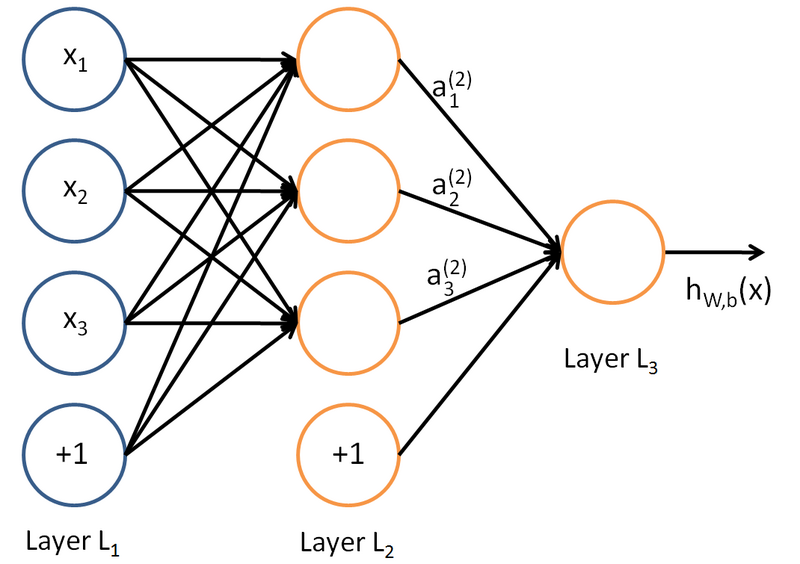
\includegraphics[width=8cm]{1.png}
\end{figure}
In this figure, we have used circles to also denote the inputs to the network.  The circles
labeled "+1" are called '''bias units''', and correspond to the intercept term.
The leftmost layer of the network is called the '''input layer''', and the
rightmost layer the '''output layer'''.The middle layer of nodes is called the '''hidden layer''', because its
values are not observed in the training set.  We also say that this example
neural network has 3 '''input units''' (not counting the bias unit), 3 
'''hidden units''', and 1 '''output unit'''.
We will let $n_l$ denote the number of layers in our network.
The neural network has parameters $(W,b) = (W^{(1)}, b^{(1)}, W^{(2)}, b^{(2)})$, where
$W^{(l)}_{ij}$ denote the parameter (or weight) associated with the connection
between unit $j$ in layer $l$, and unit $i$ in layer $l+1$.Also,$b^{(l)}_i$ is the bias associated with unit $i$ in layer $l+1$
Given a fixed setting of the parameters $W,b$,our neural network defines a hypothesis $h_{W,b}(x)$ that outputs a real number.
$$a_1^{(2)} = f(W_{11}^{(1)}x_1 + W_{12}^{(1)} x_2 + W_{13}^{(1)} x_3 + b_1^{(1)})$$
$$a_2^{(2)} = f(W_{21}^{(1)}x_1 + W_{22}^{(1)} x_2 + W_{23}^{(1)} x_3 + b_2^{(1)})$$
$$ a_3^{(2)} = f(W_{31}^{(1)}x_1 + W_{32}^{(1)} x_2 + W_{33}^{(1)} x_3 + b_3^{(1)})$$
$$h_{W,b}(x) = a_1^{(3)} =  f(W_{11}^{(2)}a_1^{(2)} + W_{12}^{(2)} a_2^{(2)} + W_{13}^{(2)} a_3^{(2)} + b_1^{(2)})$$
We call this step forward propagation.Neural networks can also have multiple output units.
Suppose we have a fixed training set $\{ (x^{(1)}, y^{(1)}), \ldots, (x^{(m)}, y^{(m)}) \}$ of $m$ training examples. We can train our neural network using batch gradient descent. In detail, for a single training example $(x,y)$, we define the cost function with respect to that single example to be:
$$ J(W,b; x,y) = \frac{1}{2} \left\| h_{W,b}(x) - y \right\|^2$$
This is a (one-half) squared-error cost function.The goal is to minimize $J(W,b)$ as a function of $W$ and $b$.We use backpropagation algorithm to minimize this cost function and get optimal set of weights to make predictions.We use the same training set to train the classifier to make predictions and record its classification accuracy on the test set.
\subsection{Sparse Autoencoders}
Suppose we have only a set of unlabeled training examples $\textstyle \{x^{(1)}, x^{(2)}, x^{(3)}, \ldots\}$,
where $\textstyle x^{(i)} \in \Re^{n}$.An autoencoder neural network is an unsupervised learning algorithm that applies backpropagation,setting the target values to be equal to the inputs.
\begin{figure}[ht!]
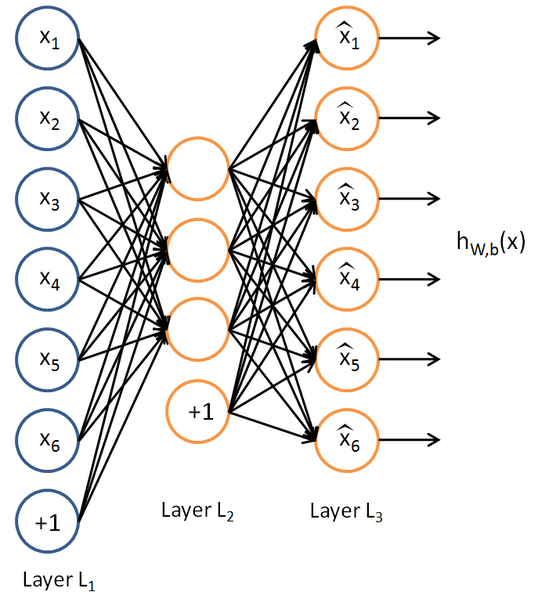
\includegraphics[width=8cm]{2.png}
\end{figure}
The autoencoder tries to learn a function $\textstyle h_{W,b}(x) \approx x $.In other
words, it is trying to learn an approximation to the identity function, so as
to output $\textstyle \hat{x}$ that is similar to $\textstyle x$.The identity function seems a
particularly trivial function to be trying to learn but by placing constraints
on the network, such as by limiting the number of hidden units, we can discover
interesting structure about the data.
Informally, we will think of a neuron as being active if its output value is close to 1, or as being inactive if its output value is
close to 0.We would like to constrain the neurons to be inactive most of the
time. 
$\textstyle a^{(2)}_j$ denotes the activation of hidden unit $\textstyle j$ in the
autoencoder.However,this notation doesn't make explicit what was the input $ x $
that led to that activation.Thus, we will write $\textstyle a^{(2)}_j(x)$ to denote the activation
of this hidden unit when the network is given a specific input $\textstyle x$.  Further, let
$$\hat\rho_j = \frac{1}{m} \sum_{i=1}^m \left[ a^{(2)}_j(x^{(i)}) \right]
$$ be the average activation of hidden unit $\textstyle j$.
We would like to (approximately) enforce the constraint
$ \hat\rho_j = \rho,$
where $\textstyle \rho$ is a sparsity parameter, typically a small value close to zero
.In other words, we would like the average activation
of each hidden neuron $\textstyle j$ to be close to 0.05 (say).To satisfy this
constraint, the hidden unit's activations must mostly be near 0.
To achieve this, we will add an extra penalty term to our optimization objective that
penalizes $\textstyle \hat\rho_j$ deviating significantly from $\textstyle \rho$.We will choose the following cost function to train sparse autoencoder and backpropagation algorithm to obtain optimal weights.
$$
\sum_{j=1}^{s_2} \rho \log \frac{\rho}{\hat\rho_j} + (1-\rho) \log \frac{1-\rho}{1-\hat\rho_j}.
$$
\subsection{Linear Decoder}
In the sparse autoencoder, we had 3 layers of neurons: an input layer, a hidden layer and an output layer.We describe a modified version of the autoencoder in which some of the neurons use a different activation function.This will result in a model that is sometimes simpler to apply, and can also be more robust to variations in the parameters. 
Each neuron (in the output layer) computed the following:
$$
z^{(3)} = W^{(2)} a^{(2)} + b^{(2)} \\
a^{(3)} = f(z^{(3)})
$$
where $a^{(3)}$ is the output. In the autoencoder, $a^{(3)}$ is the approximate reconstruction of the input $x = a^{(1)}$.
Since we used a sigmoid activation function for $f(z^{(3)})$, we needed to constrain or scale the inputs to be in the range $[0,1]$, 
since the sigmoid function outputs numbers in the range $[0,1]$.This condition can sometimes be awkward to satisfy. For example, if one uses PCA whitening, the input is no longer constrained to $[0,1]$ and it's not clear what the best way is to scale the data to ensure it fits into the constrained range.
The fix for this problem is to set $a^{(3)} = z^{(3)}$.Formally, this is achieved by having the output nodes use an activation function that's the identity function $f(z) = z$, so that $a^{(3)} = f(z^{(3)}) = z^{(3)}$. 
This particular activation function $f(\cdot)$ is called the linear activation function However in the hidden layer of the network, we still use a sigmoid (or tanh) activation function.
It is only in the output layer that we use the linear activation function. 
We use linear decoder to obtain compressed representation of features from the $8 * 8$ randomly chosen sample from a RGB image whose label is unknown to us.
 

\subsection{Deep Networks for Classification}
\subsection{Pre-Processing of Data}
Data preprocessing plays a very important in many deep learning algorithms. In practice,we have seen our performance improved between 2-7 perecent after our data has been pre-processed before using it to train a classifier.We used simple rescaling,in which our goal was to rescale the data along each data dimension (possibly independently) so that the final data vectors lie in the range $[0, 1]$ or  $[-1, 1]$.We also tried feature standardization which refers to setting each dimension of the data to have zero-mean and unit-variance. This is the most common method for normalization. We achieved this by first computing the mean of each dimension (across the dataset) and subtracts this from each dimension. Next,each dimension is divided by its standard deviation.Out of the two approaches we found z-score to perform better on RGB images.
\subsection{PCA/ZCA}

\subsection{Results}
The code\footnote{http://github.com/manishrocksag/ObjectRecognition}
for the implementation has been open sourced and can be forked. 
\subsection{References}


\bibliographystyle{ieee}
\bibliography{test}

\end{document}
